\documentclass{l4proj}

\usepackage{url}
\usepackage{fancyvrb}
\usepackage{caption}
\usepackage{placeins}
\usepackage[final]{pdfpages}
\usepackage[utf8]{inputenc}
\usepackage{listings}
\usepackage{color}
\definecolor{codegreen}{rgb}{0,0.6,0}
\definecolor{codegray}{rgb}{0.5,0.5,0.5}
\definecolor{codepurple}{rgb}{0.58,0,0.82}
\definecolor{backcolour}{rgb}{0.95,0.95,0.92}
\lstdefinestyle{code-style}{
    backgroundcolor=\color{backcolour},   
    commentstyle=\color{codegreen},
    keywordstyle=\color{magenta},
    numberstyle=\tiny\color{codegray},
    stringstyle=\color{codepurple},
    basicstyle=\footnotesize,
    breakatwhitespace=false,         
    breaklines=true,                 
    captionpos=b,                    
    keepspaces=true,                 
    numbers=left,                    
    numbersep=5pt,                  
    showspaces=false,                
    showstringspaces=false,
    showtabs=false,                  
    tabsize=2
}
\lstset{style=code-style}



\begin{document}
\title{Palgo - Algorithm Animator}
\author{Andrei-Mihai Nicolae}
\maketitle

\begin{abstract}
Understanding algorithms is both very common and hard for developers in general,
regardless of their level of expertise. Even the fundamental ones, such as Dijkstra's algorithm
for finding the shortest path between two nodes in a graph, are quite complicated to grasp. Many 
studies show that visualizing an algorithm and its steps make understanding it much easier. In
this report, we will present an Algorithm Animator built specifically for solving this problem 
in a modern, responsive and efficient manner. Among others, we will also show why certain design decisions (e.g. making it a native
desktop app instead of a basic jar, using material design for the user interface), the implementation choices and the
evaluation results make this tool a viable option for software engineers when it comes to learning different kinds of 
algorithms.
\end{abstract}

\educationalconsent

\tableofcontents
%==============================================================================
\chapter{Introduction}
\label{intro}
\pagenumbering{arabic}

Firstly, the starting point should be defining what an algorithm is.

\begin{figure}[!ht]
\centering
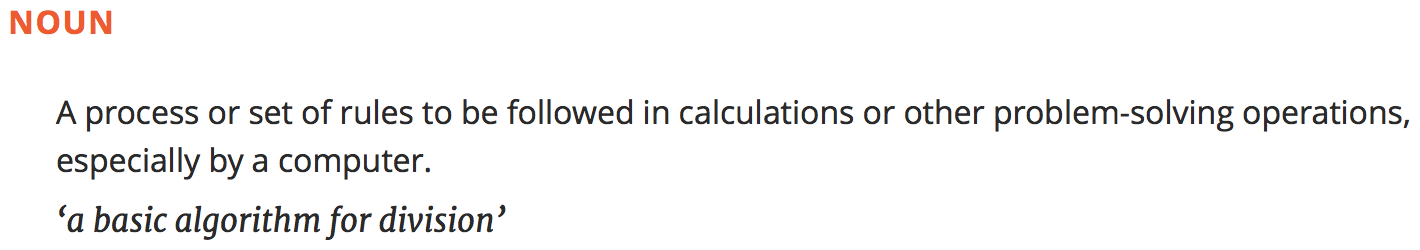
\includegraphics[scale=0.5]{algorithm}
\caption{Algorithm definition taken from the Oxford English Dictionary.}
\label{fig:algorithm}
\end{figure}

As we can see above, it is a "process or set of rules" followed by a computer when trying to solve a problem. As a machine is, at its core, composed of 1s and 0s, a human being needs to visualise what is going under the hood in order to comprehend the steps that are undertaken. In a study conducted by Cristopher D. Hundhausen et al.~\cite{av}, it was proven that even though algorithm visualisation is not the "perfect" solution, it is definitely effective in teaching students and experienced developers.

There are many tools out there that already provide this functionality, but one thing was a key factor in deciding how to proceed with planning the whole software process: there are barely any standalone applications. Even though one can find many websites which let people visualise algorithms' steps (e.g. a great example is VisuAlgo ~\cite{visualgo}), this is not such a good solution as the user cannot use the application at his/her commodity, an Internet connection being required.

Therefore, the plan was to create an app that can be run offline and would feel natural to the user regardless of the operating system of choice. There are many Java implementations (i.e. resulting in jar executables), but one of the main drawbacks is the lack of proper GUI tools that can build native-feeling applications. 

As such, the decision was made to use the Electron framework originally built by the team behind the Atom text editor. This framework uses only web tools to generate executables for all 3 main OS families (i.e. macOS, Windows and Linux) that provide the user with a native, modern and responsive feel. 

The planning was made using the best agile practices~\cite{agile-methodologies}, eventually deciding on following a variation of XP programming. Designing and coming up with an architectural plan was a major milestone to be reached as it took a considerable amount of time to be put in place. However, as it will be discussed in future chapters, the implementation of the animation engine was a crucial and time consuming challenge that required the highest amount of effort.

The report also presents how the app was test in many various ways, as well as how it was evaluated using potential end users. In the end, we shall discuss about the roadmap of the project, why open source is and will be vital for the development of the animator as well as some final thoughts and lessons learned throughout the process.

\section{Aims}

The goals of the project were set and subsequently refined throughout many project meetings, as well as meeting with some fellow classmates to get feedback along the way. 

The main aims of the Algorithm Animator, however, have always been:
\begin{itemize}
	\item Create an efficient and easy-to-use animator.
	\item Make the animator a cross-platform application that would run natively on the main operating system families: macOS, Windows and Linux.
	\item Provide a user-friendly interface that would make the user want to enjoy the product.
	\item Create at least 5-6 fully functional algorithms.
	\item Make the application scalable and easy to maintain.
	\item Test all functionality and ensure quality above quantity.
	\item Evaluate the product throughout the software process to meet acceptance criteria.
	\item Build a roadmap that would allow the animator grow even after the level 4 project has finished.
\end{itemize}

\section{Motivation}

Even if we have previously mentioned that visualising algorithms is one of the best ways of understanding how they perform, there are also other key motivational aspects behind the need of building an animator.

One such motivation is the increasing demand of software engineers throughout the industry as well as the rise in level of expertise. Developers, and students in particular, will benefit tremendously from a good grasp on how to implement correct and optimal algorithms when applying for a new job. Thus, an algorithm animator would be a good component in one's tool belt. 

Another major aspect was the opportunity to create a modern tool that would make users enjoy working with it. At the moment, one of the most popular animator toolkits is the one presented in John Morris' paper~\cite{animator-toolkit}.  Below a screenshot was taken from the app. \newpage

\begin{figure}[!ht]
\centering
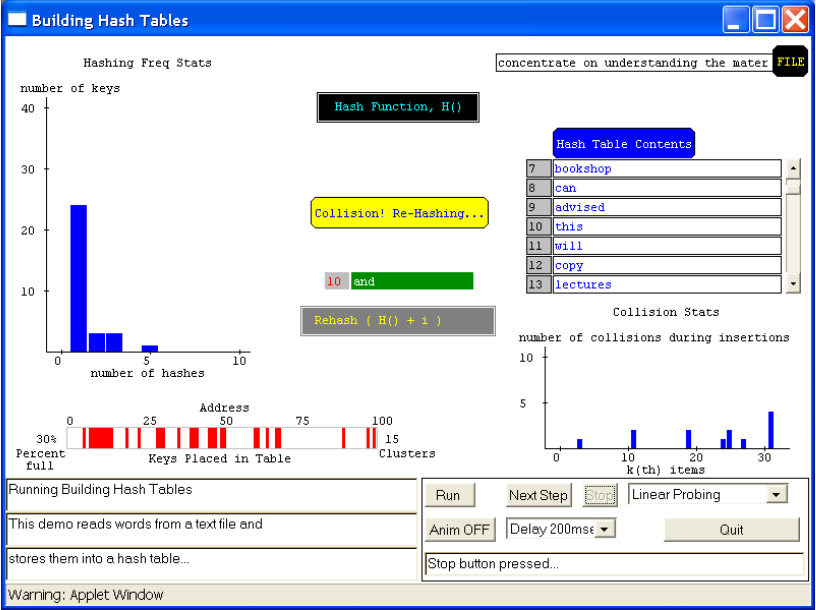
\includegraphics[scale=0.8]{animator-toolkit}
\caption{John Morris' Animator Toolkit.}
\label{fig:animator-toolkit}
\end{figure}

It was written in Java, which comes with certain advantages: multi-threading support, enhanced familiarity due to university coursework and projects etc. However, the lack of proper graphical user interface components makes this a not so viable option for regular users when adopting it.


\begin{figure}[!ht]
\centering
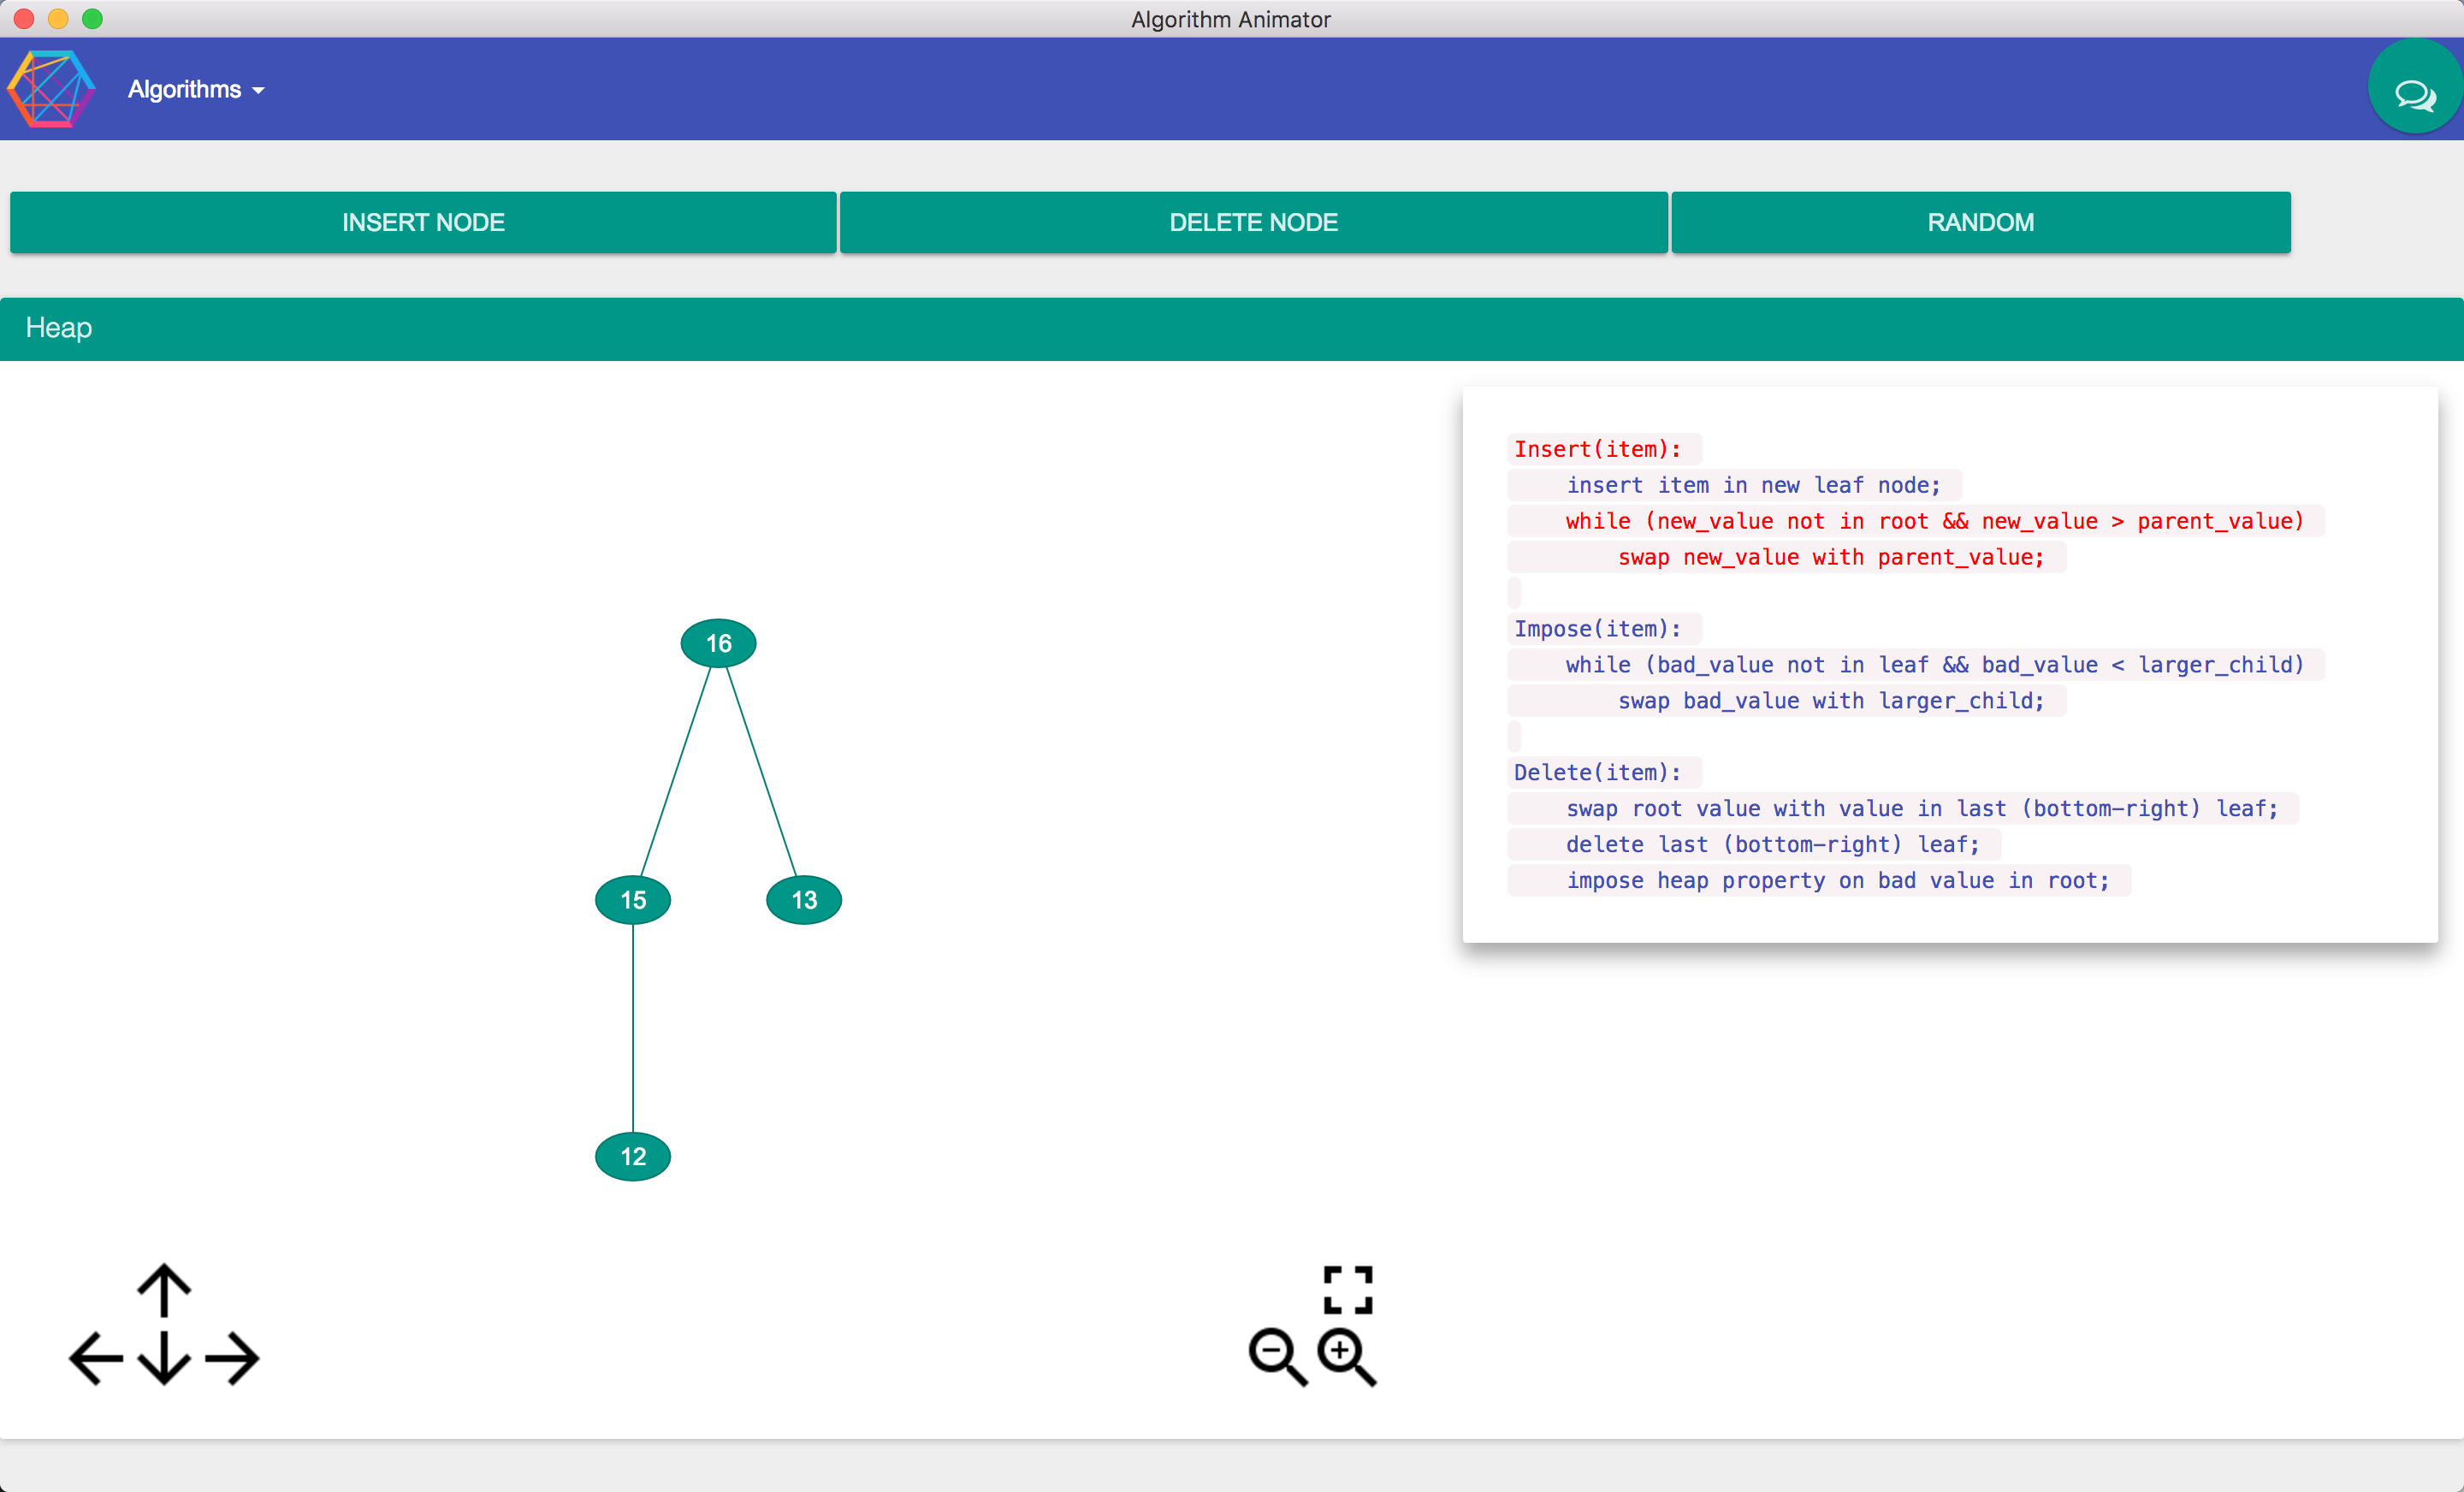
\includegraphics[scale=0.3]{algo-animator}
\caption{The animator presented in this report.}
\label{fig:palgo}
\end{figure}

We can see a clear difference between the two and why one might choose the latter option due to familiarity (native feel) and easy-to-use user interface.

\section{Contributions}

This report serves to deliver certain main contributions:

\begin{itemize}
	\item Shows the whole software development lifecycle of an algorithm animator.
	\item Presents various technologies used to build native and modern desktop apps~\cite{electron}~\cite{visjs}
	\item Provides a brief overview of current animators available and background knowledge on their benefits and efficiency in teaching.
\end{itemize}


\section{Report Content}
The rest of the report will analyse the background of animators and why they were proven useful, as well as cover all the steps in gathering requirements, designing, implementing, testing and evaluating the tool. 

\begin{itemize}
\item Chapter~\ref{background} covers work related to the purpose of algorithm animators and why they are useful 
\item Chapter~\ref{requirements} goes into how the problem was analysed and what requirements were gathered through
	project meetings and discussions with Algorithmics students.
\item Chapter~\ref{project-management} shows the steps undertaken to follow the best agile methodology principles.
\item Chapter~\ref{design} explains the design decisions behind the tool and illustrates various lessons learned and
	problems faced along the way.
\item Chapter~\ref{implementation} goes into the implementation details of the animator.
\item Chapter~\ref{testing} show how extensive unit, integration and other types of testing (e.g. smoke, end-to-end)
	were undergone and why they were essential to the development of the application.
\item Chapter~\ref{conclusions} details the overall results of the project.
\end{itemize}

%==============================================================================

\chapter{Background}
\label{background}

Firstly, we need to define an algorithm. We will use the above-mentioned definition taken from the Oxford dictionary~\cite{oxford-dict}: "A process or set of rules to be followed in calculations or other problem-solving operations, especially by a computer". In our case, we will only relate to set of rules followed solely by computers. Thus, put simply, an algorithm is a set of steps defined by someone in order to solve some problem. As an algorithm can be written by anyone, there is no known number or catalog of them. However, the most important algorithms (e.g. Huffman tree encoding/decoding) are taught in any Computer Science course at universities around the globe.

Having defined what an algorithm is, let's take an actual example - Dijkstra's algorithm for finding the shortest path between two nodes~\cite{dijkstra-shortest-path}, first published almost 60 years ago (the pseudocode was formally checked by Dr. Norman):

\begin{lstlisting}[language=Java, caption=Pseudocode for Dijkstra's shortest path algorithm]
// S is set of vertices for which shortest path from u is known
// d(w) represents length of a shortest path from u to w
// passing only through vertices of S
S = {u}; // initialise S
for (each vertex w) d(w) = wt(u,w); // initialise distances
while (S != V) { // still vertices to add to S find v not in S with d(v) minimum;
	add v to S;
	for (each w not in S) // perform relaxation
	d(w) = min{ d(w) , d(v)+wt(v,w) };
}
\end{lstlisting}

As one might observe, this is not trivial to grasp. Therefore, many solutions have been created in order to help students and engineers in general understand them better. One such solution is a rather creative one, developed by students at Spatienta University, which tries to teach different sorting algorithms by dancing.

\pagebreak

\begin{figure}[!ht]
\centering
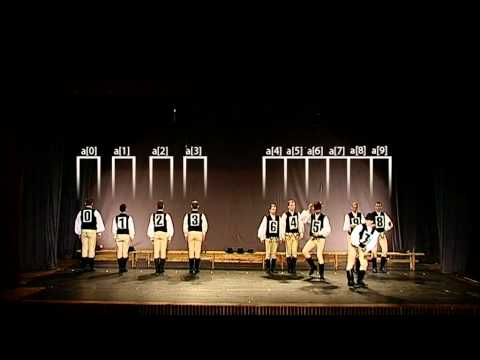
\includegraphics[scale=0.6]{quicksort}
\caption{Sorting algorithms learning through Hungarian folk dancing.}
\label{fig:quicksort}
\end{figure}

This was featured on many websites and gained enormous traction among computer science enthusiasts. However, a more traditional approach that is adopted formally in universities as well is the use of animators.

Firstly, let's define what an animator is. Again, taking the definition from the Oxford dictionary~\cite{oxford-dict}, it is "a person who makes animated films". In our case, the person is the computer and the film is the sequence of steps required to produce an output after feeding input to an algorithm. 

Usually, most algorithm animators are divided into 2 sections: one side will contain the graphics in order to represent the data structures used (e.g. in graph traversal algorithms the nodes and edges comprising the graph will be drawn) while the other side will have the code lines, the actual rules the computer needs to follow in order to produce the desired output. In general the current code line that is executed at a certain moment is highlighted, while the data structure visualized (e.g. some box that represents an array's element) changes and the user can see the output visually and immediately, making a mental connection between the code line and the change it produces. 

But why an animator precisely? There are many studies that show visualization in any area can enhance learning capabilities drastically. Brenda Parker and Ian Mitchell's work~\cite{parker-mitchell} shows clearly how seeing the steps can greatly improve a student's understanding of what is happening "behind the scenes". On the other hand, even if animations were proven to be generally useful and beneficial for the learner, the need for seeing algorithms animated declines over time, as the study shows. 

Another study by Susan Palmiter and Jay Elkerton~\cite{palmiter-elkerton} tried to find out which method was the most effective in learning new computer-based tasks. Even though animations for complex mechanisms were found not to be as effective as for some easier one (e.g. parallel programming vs. graph traversal), they are very helpful for the algorithms generally taught at university courses or used most often.

Having discussed methods of learning new algorithms better and why animators are useful, we need to take a look at previous solutions developed by other people. Apart from John Morris' tool shown above, there are many other applications available, including Galant~\cite{galant} and the visualizer built by D. Galles~\cite{galles}.

\pagebreak

\begin{figure}[!ht]
\centering
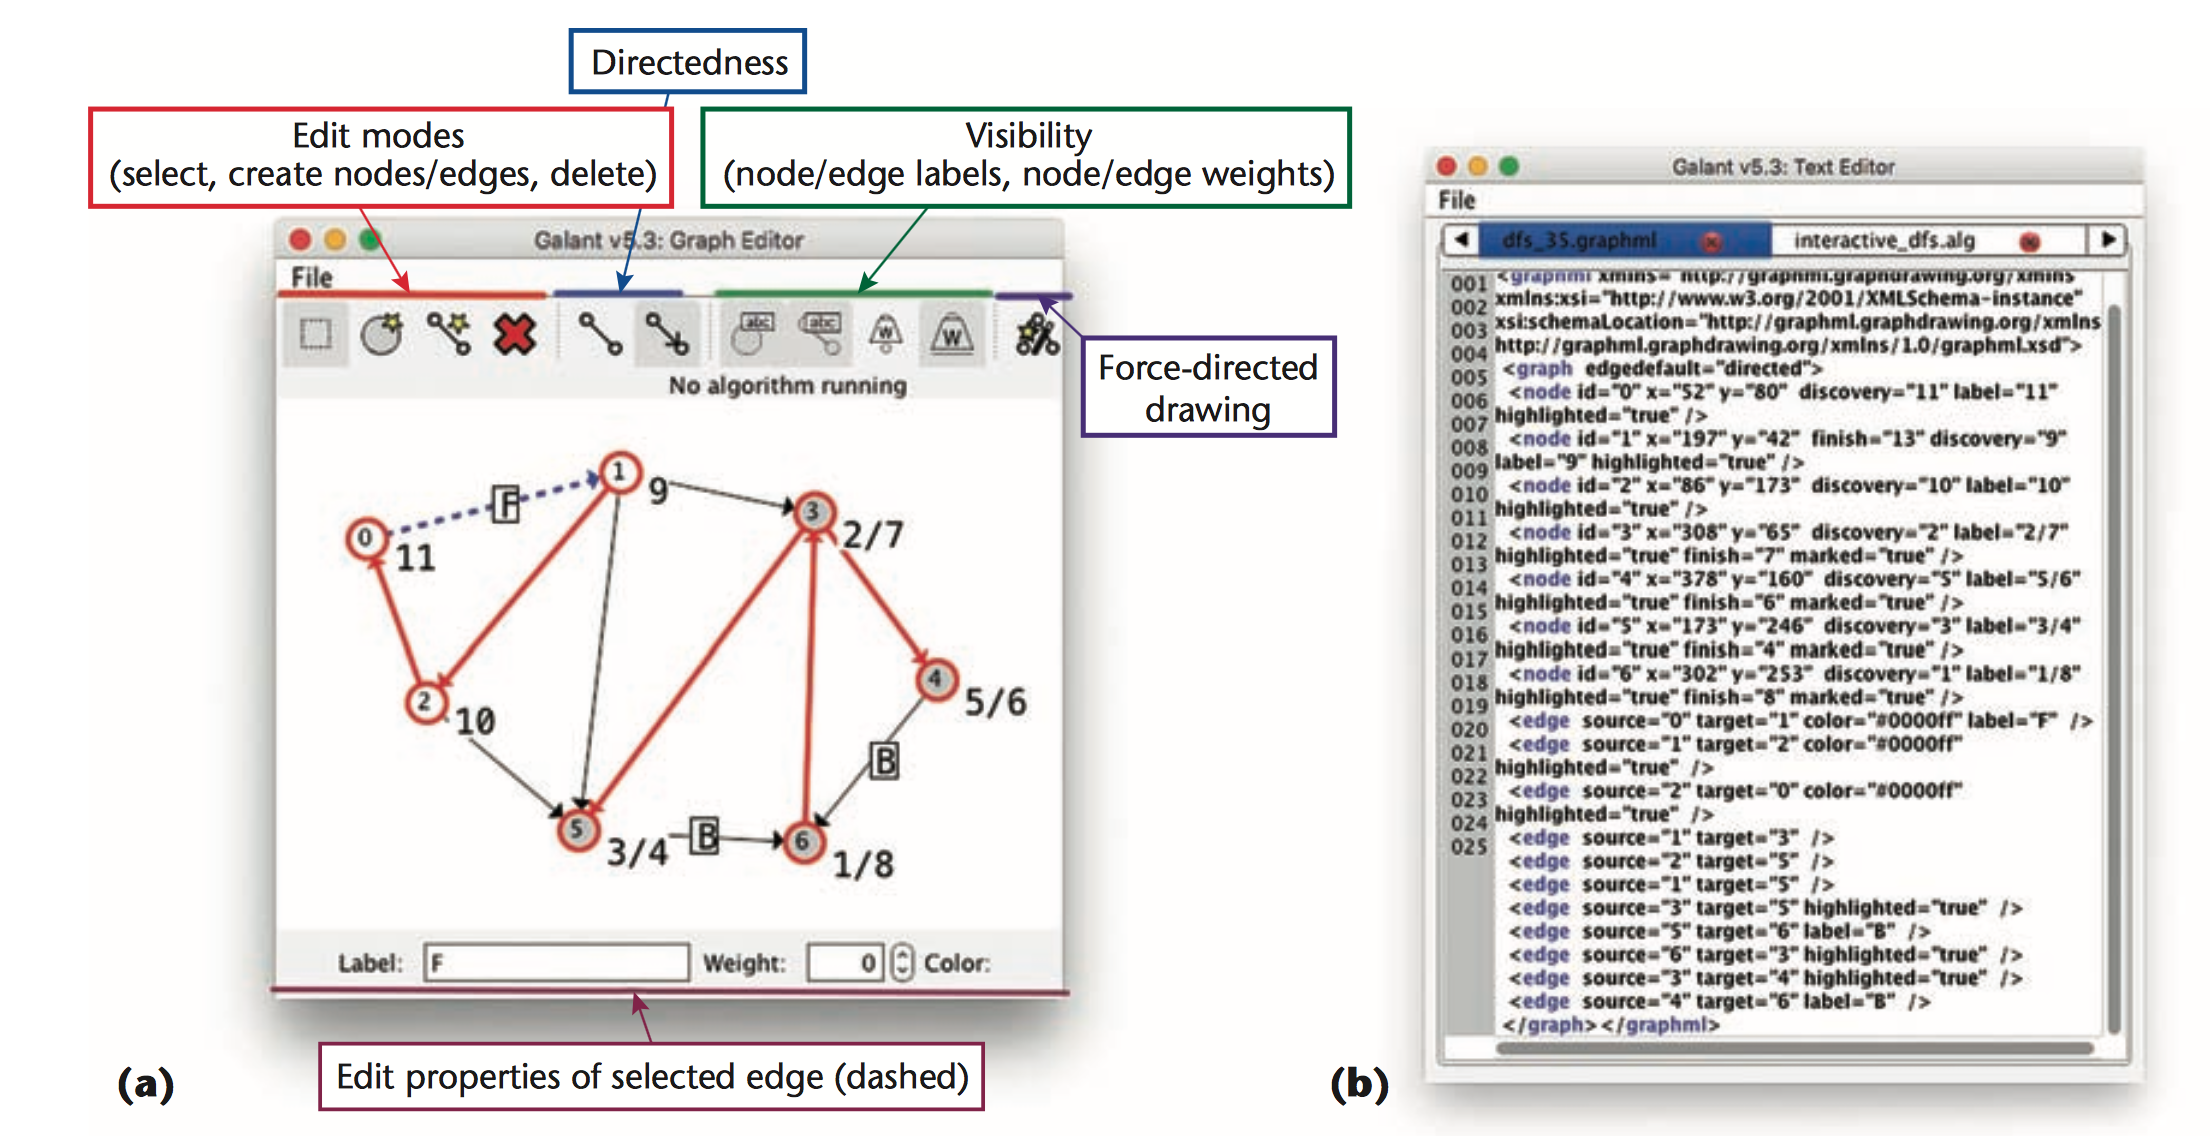
\includegraphics[scale=0.4]{galant}
\caption{Galant Algorithm Animator.}
\label{fig:galant}
\end{figure}

Here we can see one of the 2 main approaches of building an animator, which is a standalone JAR application. Thus, it is written completely in Java and, as the language is pre-installed on most electronic devices, it can run on the major operating systems families. 

There are obvious advantages to this approach:
\begin{itemize}
	\item end product can run on a variety of machines with only one codebase
	\item large number of Java libraries facilitate an easy development workflow
    \item many tutorials and resources available
    \item java is taught at most universities in introductory courses, making it easier for newcomers to create their own application rapidly
    	\begin{figure}[!ht]
		\centering
		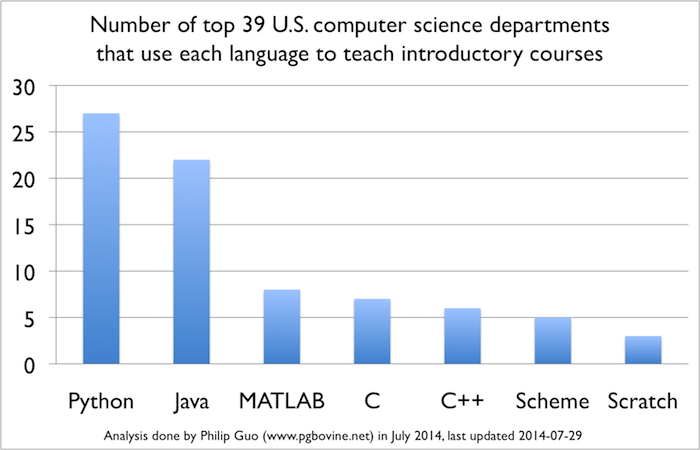
\includegraphics[scale=0.8]{java-uni}
		\caption{Languages used in introductory courses at top US universities.}
		\label{fig:java-uni}
		\end{figure}    
\end{itemize}

\pagebreak

However, there are also drawbacks:
\begin{itemize}
\item the most popular Java libraries for producing standalone graphical JAR applications output old-fashioned user interface
\item the code for drawing on the canvas and animating in Java (using Swing or JavaFX) can become extremely verbose and unreadable
\end{itemize}

On the other hand, we also have the web approach to building animators, one of them being D. Galles' application~\cite{galles}.

\begin{figure}[!ht]
\centering
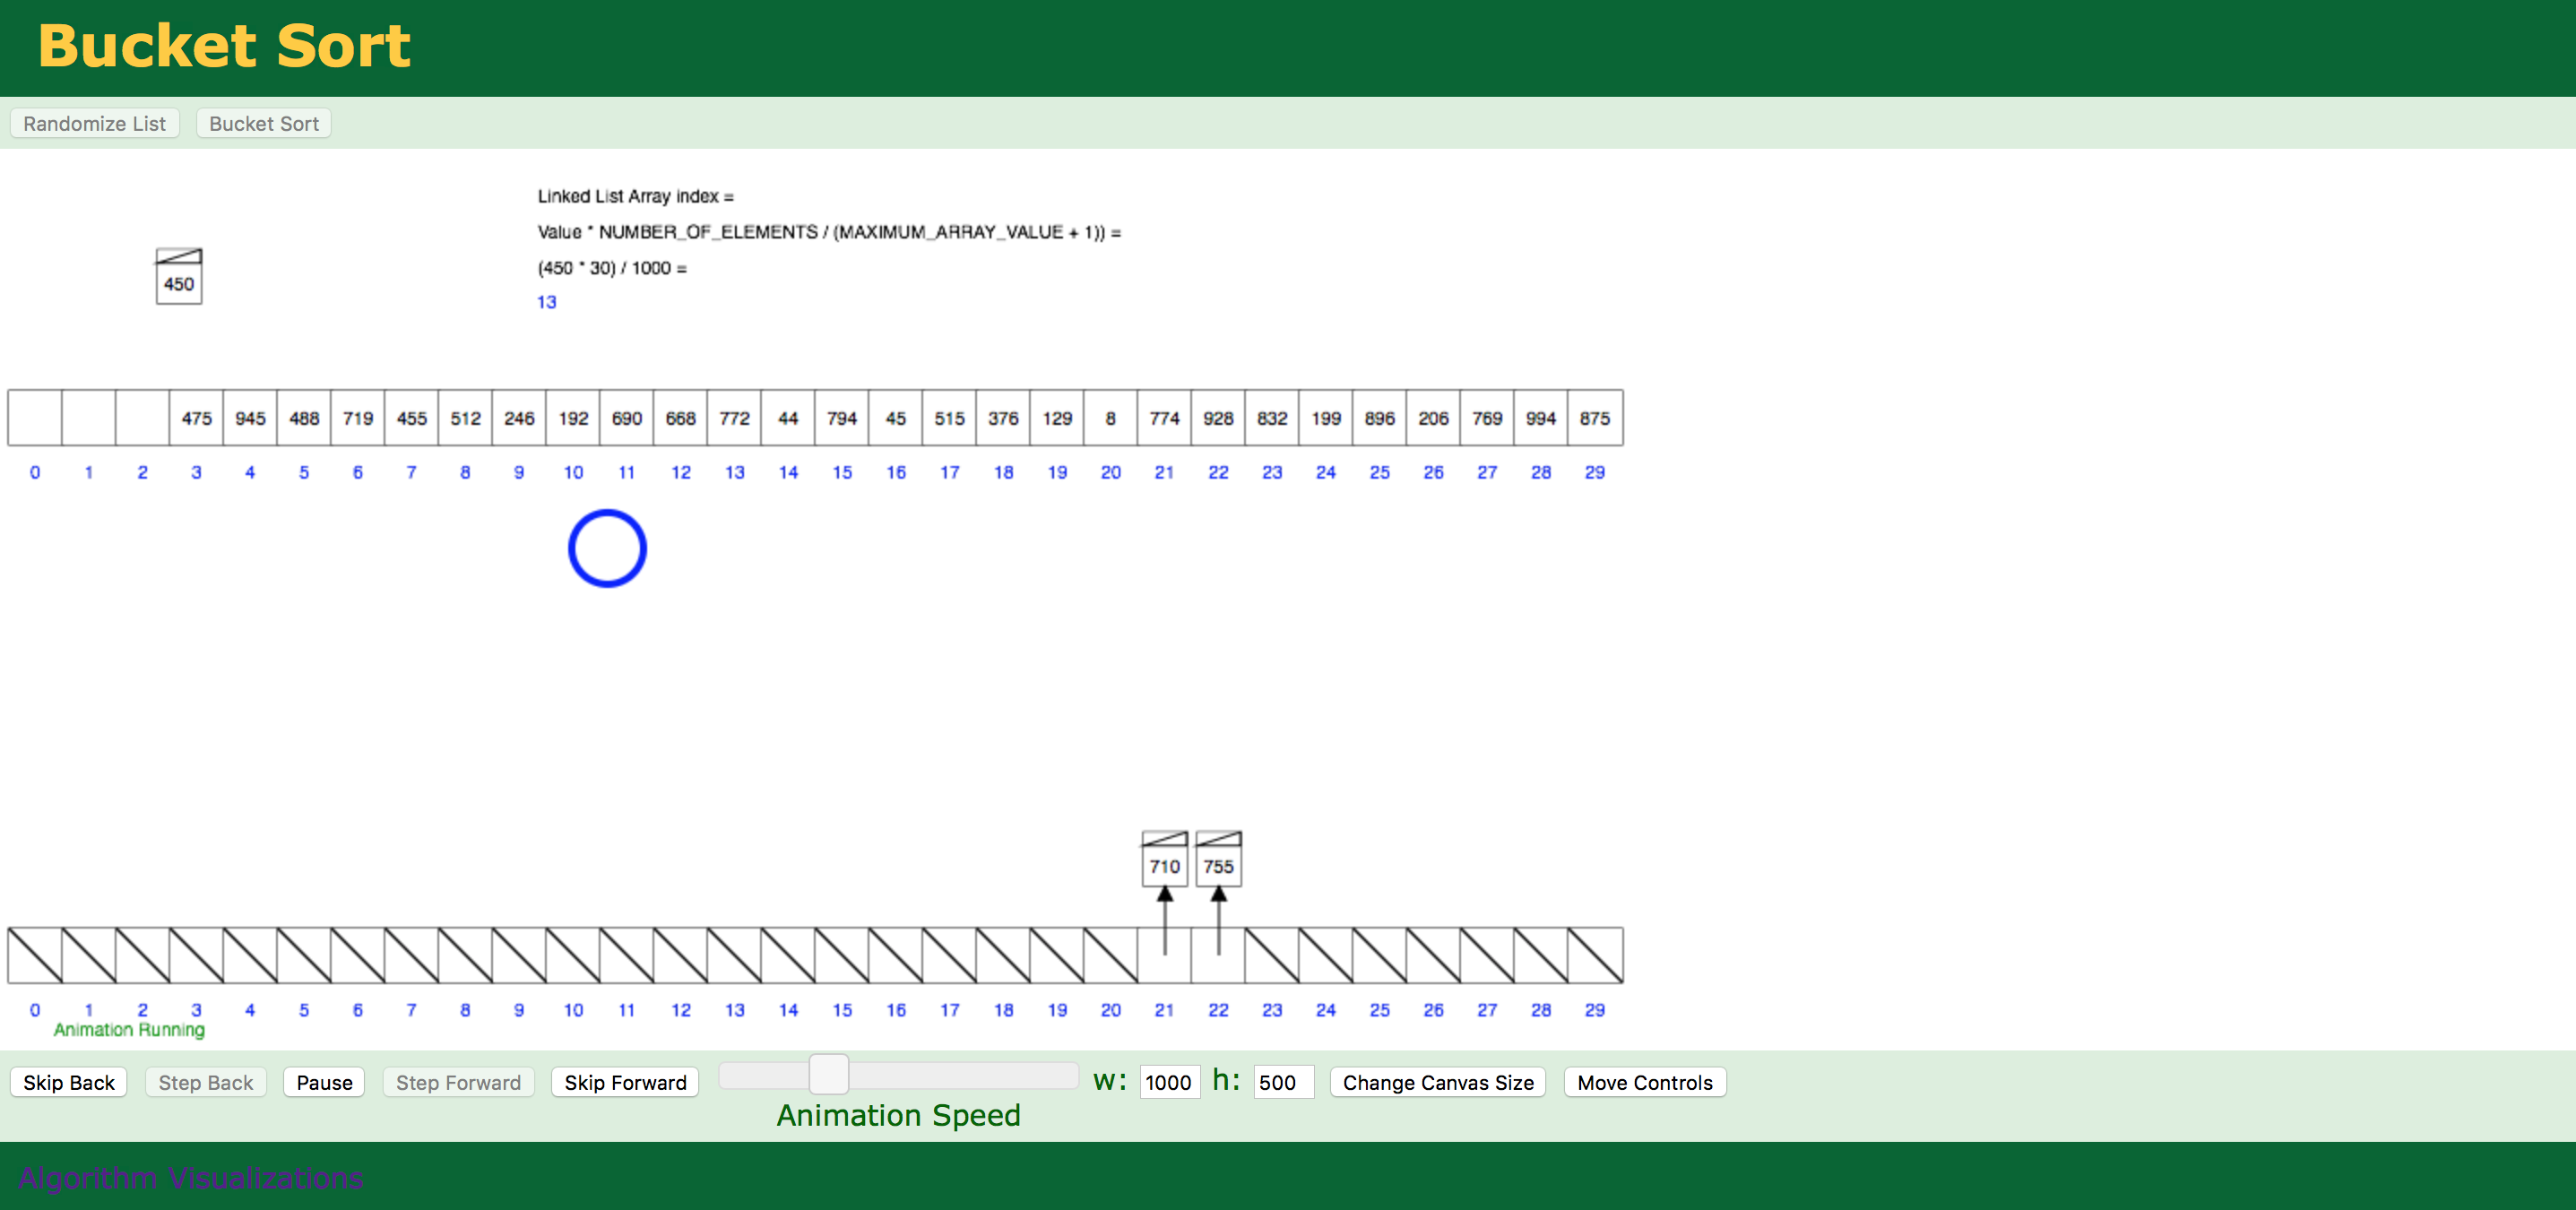
\includegraphics[scale=0.25]{galles}
\caption{Algorithm animator built by D. Galles at University of San Francisco.}
\label{fig:galles}
\end{figure}

Some advantages of this solution are the following:
\begin{itemize}
\item the developer can use a wide variety of JavaScript tools (e.g. drawing directly on HTML5 canvas, VisJs, SigmaJs) to draw and animate objects
\item the app can have a very modern and responsive feel which can make users enjoy the product
\item virtually all users have at least a browser installed on their machine, thus making the animator available to everyone 
\end{itemize}

However, the main drawback is that it is still a website, thus it need to be hosted (which implies additional costs) and it cannot be reached by anyone at all times due to the fact that not everyone has constant Internet access.

We have covered all the necessary background and related work before diving into how Palgo was designed and implemented. We believe that our solution is a combination of the two main approaches listed above, merging the benefits of both into a single tool.

%==============================================================================

\chapter{Requirements}
\label{requirements}

As for every software built with best practices, requirements need to be gathered, defined, analyzed and then prioritized. As we tried to follow an Agile structure, the requirements have changed every week through student-supervisor weekly as well as end user meet-ups. 

We tried to keep the requirements SMART~\cite{smart-requirements}, which implies they are specific, measurable, attainable, realizable and time bounded. Thus, making them follow this well established format made the software development lifecycle much faster and cleaner.

Below is a screenshot from a Trello~\cite{trello} board used during one of the iterations (a separate board was used for tracking non-functional requirements as well).

\begin{figure}[!ht]
\centering
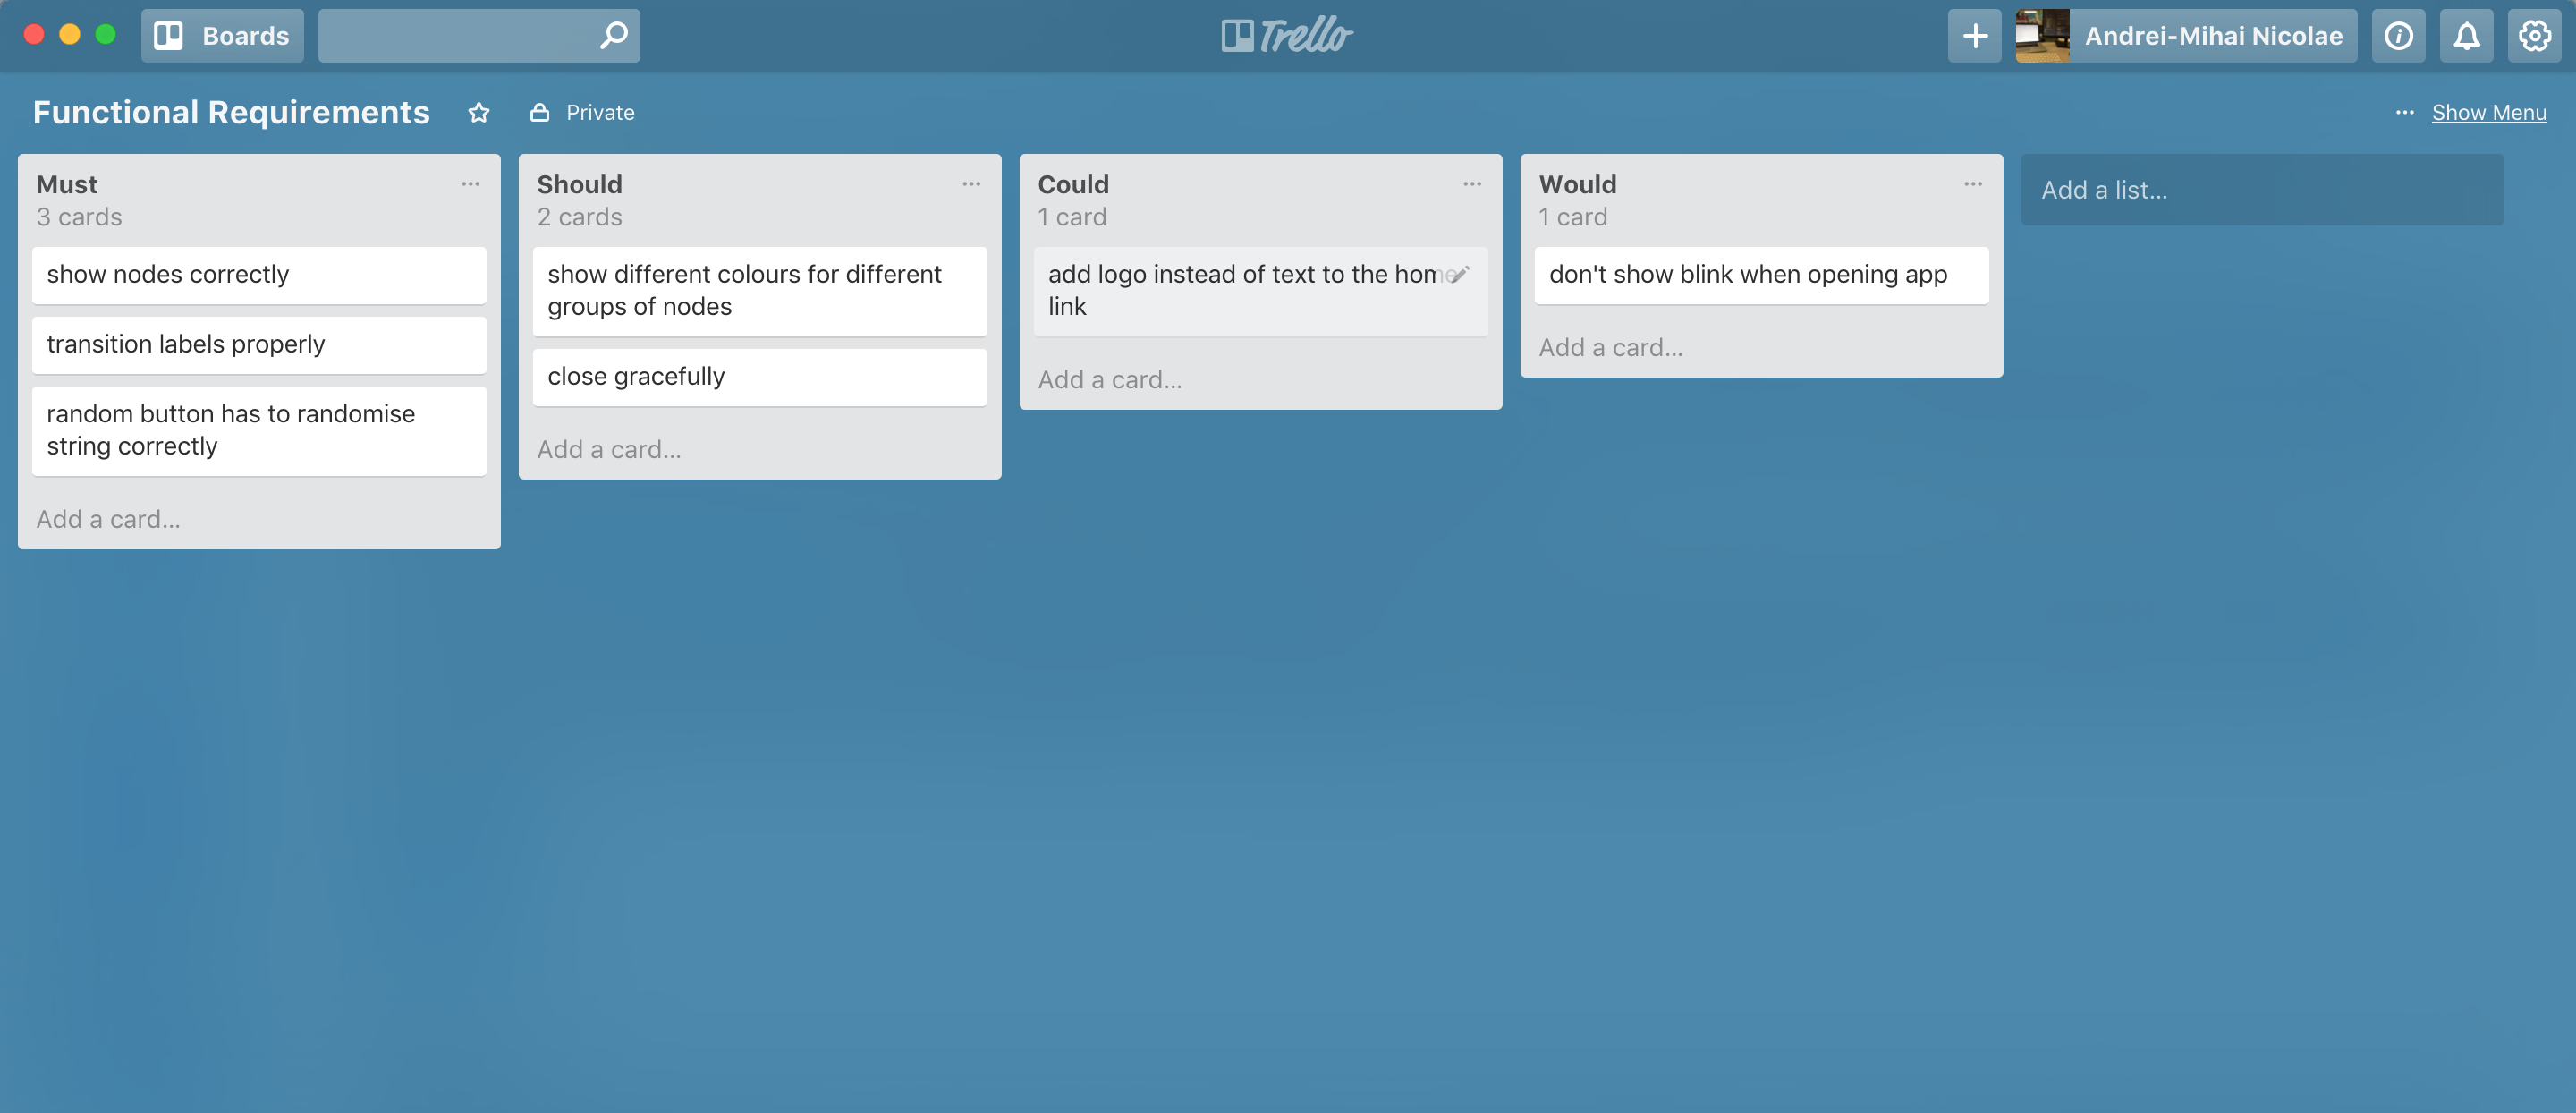
\includegraphics[scale=0.35]{trello-functional-requirements}
\caption{Trello board for functional requirements during one of the iterations.}
\label{fig:trello-functional-requirements}
\end{figure}

The requirements followed a pipeline through which the requirement together with its rationale would get broken down into pieces continuously until user stories would be produced. One example of such a requirement would be: "Show me a correct and easy-to-understand animation for the insert function in a heap data structure.". This would then be broken down in multiple user stories, such as "Color current node that is inserted and add its label" and "Highlight code line corresponding with changing the label". 

We also tried to follow the MoSCoW~\cite{moscow-requirements} guideline for prioritizing the requirements. The technique has proven to be very effective and it is adopted widely in industry, even though the paper is more than 20 years old. This facilitated a smooth workflow and concise goals to be targeted.

\section{Problem Analysis}

We have analyzed the problem systematically, devising it into multiple main questions to be answered:

\begin{itemize}
\item who are our target users?
\item what type of format will the application have (i.e. web/desktop)?
\item what algorithms should be animated?
\item how would the main layout be structured?
\end{itemize}

During the analysis, we needed to take into account various factors, including how much experience with algorithms and computer science in general will our users have or what algorithms would need visualization the most. As previous animators built under the supervision of Dr. Norman are used for educational purposes in the level 3 Algorithmics I course, we believe that having mainly graph and tree algorithms would benefit the project the most. However, we tried to keep the structure simple and the codebase easy-to-maintain such that other families of algorithms will be straightforward to implement. Because we want to project to be continued in the open source space, users other than students can use the animator, thus we tried to keep the requirements more general.

Also, there was much discussion around whether to use a web or a desktop approach. For reasons explained above, we resumed to implementing a desktop application using the technologies mentioned in the subsequent chapters.

We have gathered requirements and split them into functional and non-functional ones, dividing them further into smaller tasks to be implemented. At the end, we were left with user stories that could be translated directly into work tasks.

\section{Requirements Gathering}

As mentioned above, the requirements gathering was a continuous process that lasted from first week of 4th year up until the end of the project's development lifecycle. Not only that we had the weekly regular student-supervisor meetings were we could add or refine requirements, but there were also meetings with possible end users.

Every two or three weeks there were meetings scheduled with a couple of classmates from University of Glasgow's Computer Science course that would give continuous feedback after testing the newest version of the application. We met in one of the laboratories in Boyd Orr building where they were provided with an executable that could be run on their personal laptops. They were given around 15 minutes to try the features and, afterwards, they provided invaluable feedback without which the animator would not perform as efficiently as it does today.

\section{Functional Requirements}

Functional requirements target specific functionalities that the system should perform. They started with a couple of algorithms that needed to be animated. Then, functionalities such as current code line highlighting and specific button behaviors began to stack up. Eventually, we can categorize them as follows:

\begin{itemize}
\item animate tree/graph depending on what the user chose to do (e.g. insert/delete node)
\item highlight current code line for every algorithm
\item define specific behavior for every button displayed on the UI
\item each window interaction should perform as expected depending on the operating system the user is using the application on
\end{itemize}

Many smaller ones appeared along the software process, but the above mentioned are the main categories.

\section{Non-Functional Requirements}

A non-functional requirement is a type of requirements that judges the system as a whole and how it operates rather than checking for specific criteria. The main non-functional requirements were rather set from the beginning. We decided to have an algorithm animator that would:

\begin{itemize}
\item be easy to use and let the users familiarize rapidly
\item make users enjoy playing with the product
\item be installed/fetched with ease
\item allow end users to use it on any platform
\item be efficient and not consume excessive resources
\item be maintainable and scalable (i.e. let future possible contributors add algorithms easily)
\end{itemize}

%==============================================================================

\chapter{Project Development}
\label{project-management}

Good software practices are key to successful projects. We have followed Agile methodologies, especially what was taught last year in the Professional Software Development class, as well as through Ian Sommerville's "Software Engineering" book~\cite{software-engineering}. 

\section{Extreme Programming}

We have followed the approach first coined by Kent Beck called Extreme Programming~\cite{extreme-programming}. It is an Agile technique through which good practices are most times pushed to "extreme" levels. XP has proven to be very effective as many companies in the industry use it in their development lifecycle. Some principles it promotes which we have followed are:

\begin{itemize}
\item frequent releases based on requirements gathered incrementally in meetings (e.g. supervisor-student meetings)
\item constant refactoring to promote simplicity
\item customer involvement throughout the whole process
\item people over processes, which means collective ownership of the code as well as avoiding exhausting long working hours
\end{itemize}





\section{Planning}

\section{Continuous Integration}

\section{Refactoring \& Incremental Planning}

\section{Issues \& Bug Tracking}

%==============================================================================

\chapter{Design}
\label{design}

\section{Architecture}

\subsection{EDA (Event-driven Architecture)}

\section{Native Desktop App vs. Jar}

\section{Electron}

\section{Vis.js}

\section{Material Design}

\section{Compromises}

%==============================================================================

\chapter{Implementation}
\label{implementation}

\section{Project Structure}

\section{JavaScript and Multi-Threading}

\section{JS Animation Engine}

\section{Extra Features}

\section{Lessons Learned}

\section{Issues Faced}

%==============================================================================

\chapter{Testing}
\label{testing}

\section{Unit Testing}

\section{Integration Testing}

\section{Prototype Evaluation}

\section{Results}

%==============================================================================

\chapter{Conclusions}
\label{conclusions}

\section{Open Source}

\section{Project Roadmap}

\section{Final Thoughts}

\section{Acknowledgements}

\bibliographystyle{plain}
\bibliography{l4proj}
\end{document}
